\graphicspath{{figure/maegaki}}
\section*{あとがき}\addcontentsline{toc}{part}{あとがき}\vspace{-1.25em}
\subsection*{作れた？}
さてみなさん、この本でVVVFインバータは作れたでしょうか？\par
もし作れたなら、ぜひ感想をください！TwitterのDM、boothのメッセージ、gmailなど、なんでもいいです。感想は次の本を書くモチベーションになりますし、単純に嬉しいです。\par
もし作れなかったなら、どこがわからなかったか、難しかったか、ぜひ教えてください。次の本や改訂版の参考にします。
また、VVVFインバータを作った人は、個人ブログやTwitterで「\#VVVFインバータの創り方」や「\#淫技」をつけて投稿してください。僕もエゴサで見に行きますし、他の人も見ると思います。みんなでVVVFインバータを作って、パワエレの楽しさを共有しましょう。
\subsection*{次の本は？}
予定では、次はPvくん担当で「コンバータの創り方」を書くことになっているそうです。多分PFCとかDCDCの話になると思います。僕は高専4年でこれから大学編入があるので、イラストだけ担当とかになりそうです。まあ、頑張ります……。（今までマトモにそういう勉強したことないのでどうしよう……。）
\subsection*{ウラバナシ①: C106は？？}
前回、約1年前にC105で2024年12月号を出してから新刊を出していませんでした。つまりC106が空白だったわけです。C106も新刊を出す予定でしたが、バカすぎて出店の予約を忘れたのです。そんなら時間空いた分C107にゼロから書いて大作？を出すのもありだろうと、今回のC107があるわけで…。結論、僕が社会不適合者なのでC106は欠番です。ごめんなさい。
\subsection*{ウラバナシ②: 編集環境について}
さて、今回も組版には\LaTeX を使っています。この\LaTeX ってのを出せるのが\LaTeX である何よりの証拠で\LaTeX 。C104から引き続き\LaTeX で運用しています。今回から、styを全部作り直していい感じになりました。従来のstyだと、文章流し込みによる改ページがされると虚無が出力されるという絶望的なエラーがありました。C105でしばしば妙な空白があったのは\texttt{\string\clearpage}を使ってこれを回避していたためです。C107ではこのエラーはもちろん解消済みです。
\\\\\textbf{〈IR2110〉（編集者兼著者兼イラスト担当）}
\newpage
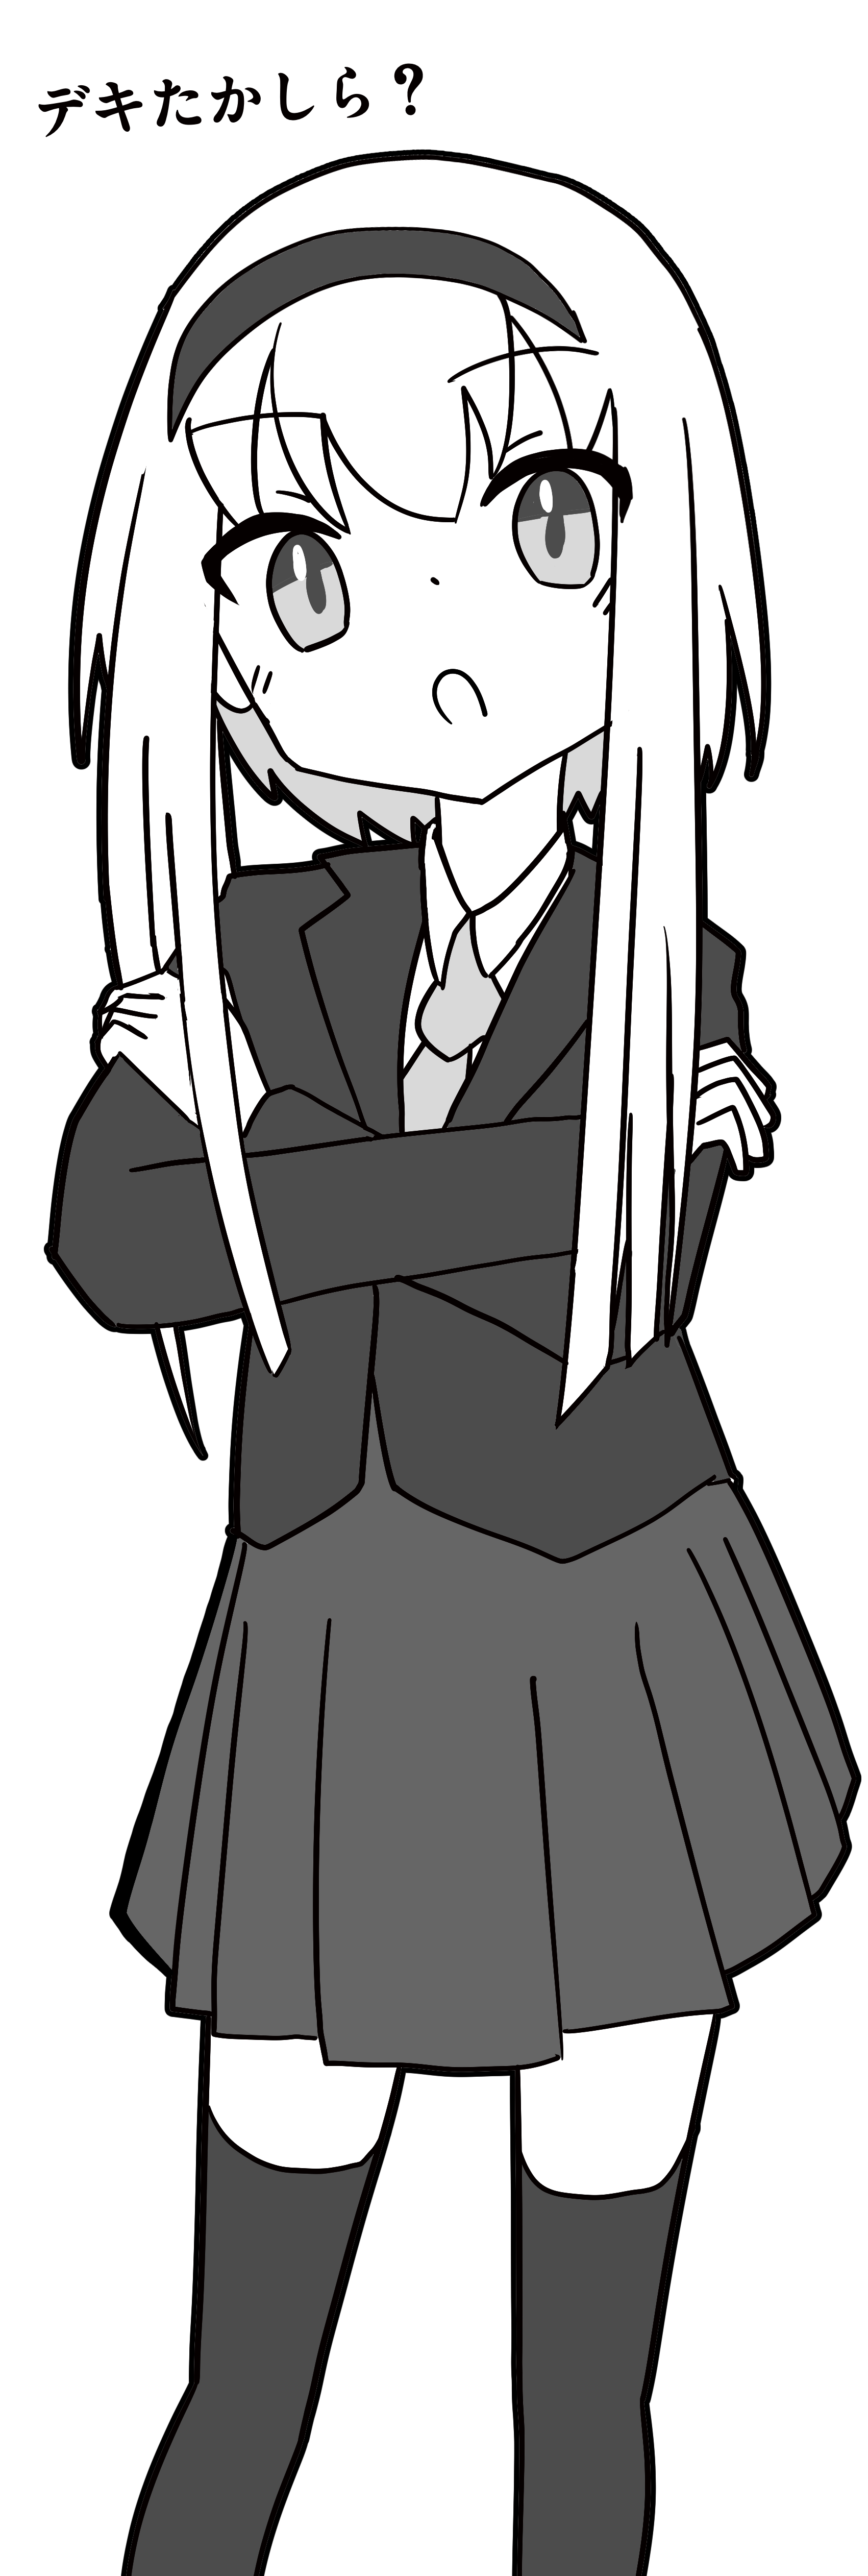
\includegraphics[width=72mm]{あとがき.png}